\section{Results}
\label{sec:modelling_results}

Our goal for this new model is to improve the accuracy of the deformable object motion model (for use in the controller in Sec.~\ref{sec:stretching_constraint_controller}), while maintaing reasonable computation speed. As mentioned in previous sections, our benchmark model is \cite{Berenson2013} (Sec.~\ref{sec:diminishing_rigidity}). To evaluate our method we perform experiments in simulation and on a physical robot. The simulator used is Bullet physics \cite{Coumans2010}, however, we emphasize that our method has no knowledge of the simulation parameters or simulation methods used therein. The simulator is used as a ``black-box,'' mainly to stand in for a perception system and to allow us to do repeatable experiments. The physical robot consists of two KUKA iiwa 7DoF arms with Robotiq 3-finger hands.

We ran experiments with scenarios involving both cloth and rope. The parameters are set as $\drkdir = 4$, $\drkdist = 10$, $\drkrot = 20$ for the new model. The parameters we used for the benchmark method are its default best value found in \cite{McConachie2018}. All experiments were run on a i7-8700K 3.7 GHz CPU with 32 GB of RAM. A video showing the experiments is included with this paper.
\todoin{Fix "included with this paper" comments throughout}

\subsection{Simulation Environment Model Accuracy Results}
% \label{Results:accuracy}

\begin{figure}[ht]
    \centering
    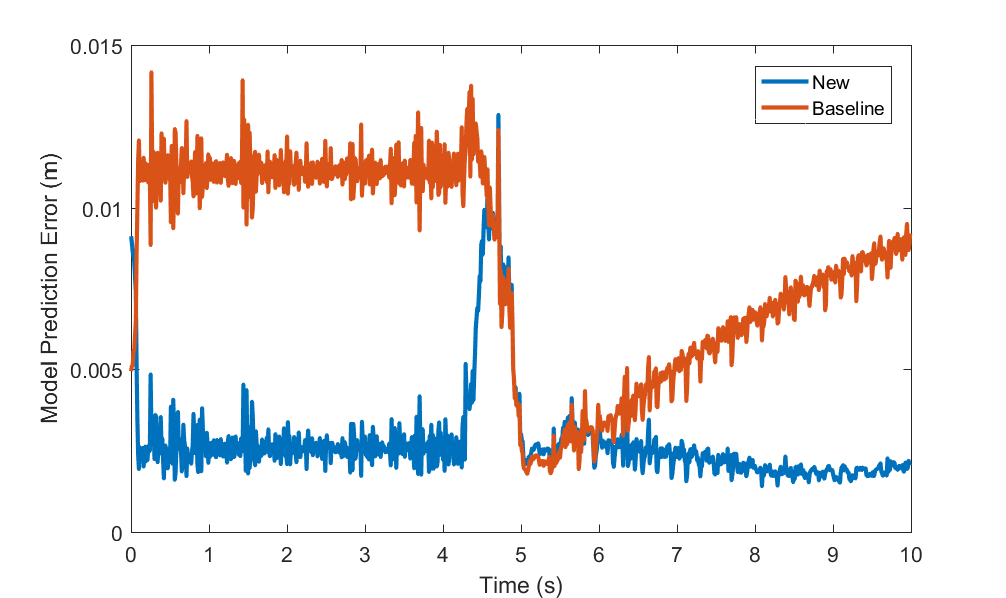
\includegraphics[width=0.85\columnwidth]{rope_model_accuracies.png}
    \caption{RMS model prediction error for the simulated rope model accuracy test. The gripper pulls the rope for the first 4.5 seconds, then turns for half a second, then moves in the opposite direction at the 5 second mark.}
    \label{fig:rope_model_accuracy_plot}
\end{figure}

\begin{figure}[ht]
    \centering
    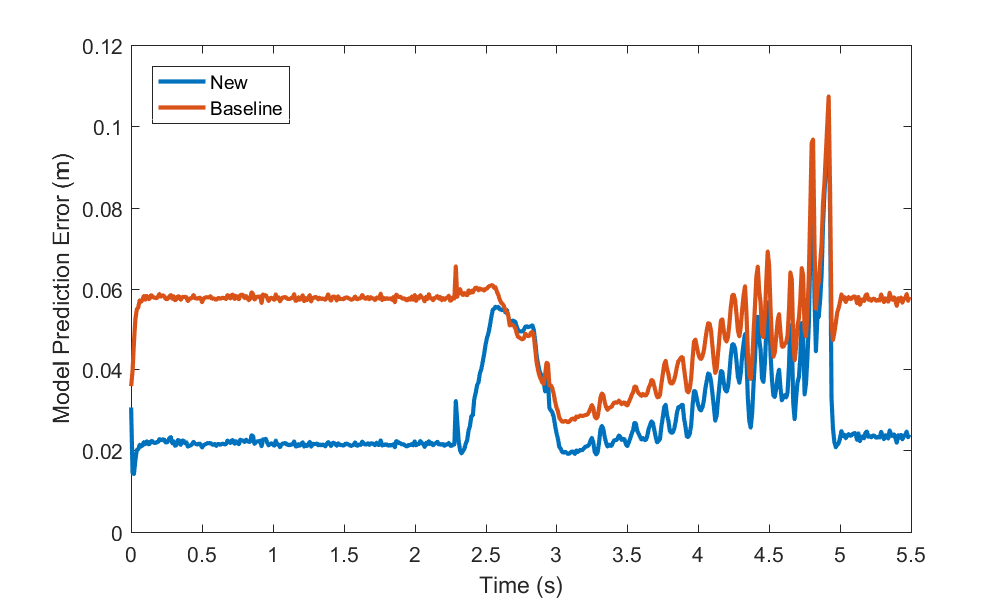
\includegraphics[width=0.85\columnwidth]{cloth_model_accuracies.png}
    \caption{RMS model prediction error for the simulated cloth model accuracy test. The grippers pull the cloth for the first 2.3 seconds, then turn for 0.63 seconds, then move in the opposite direction at the 2.93 second mark. At the 5 second mark the cloth is no longer folded. }
    \label{fig:cloth_model_accuracy_plot}
\end{figure}

We evaluated model accuracy by pulling the rope in a straight line along the direction of the rope, then turning the gripper and pulling back towards the rope as shown in Fig.~\ref{fig:intro_directional_rigidity}. As shown in Fig.~\ref{fig:rope_model_accuracy_plot}, our new model is a better approximation of the true motion when the gripper is pulling the rope. When the gripper is turning, both the baseline and the new model produce comparable error, but when the gripper starts pulling again (this time in the opposite direction), the new model is a significantly better approximation.

We also evaluated model accuracy by pulling the cloth in a similar fashion; pulling the cloth one way, turning the grippers, and then pulling in the opposite direction. As shown in Fig.~\ref{fig:cloth_model_accuracy_plot}, our new model is a better approximation of the true motion when the grippers are pulling the cloth. As in the rope test, when rotating the grippers both models produce comparable error. While the cloth is folded on itself both models produce noisy results, but when the cloth lies flat again, the new model achieves lower error.



\subsection{Physical Robot Experiments}

\begin{figure}[ht]
    \centering
    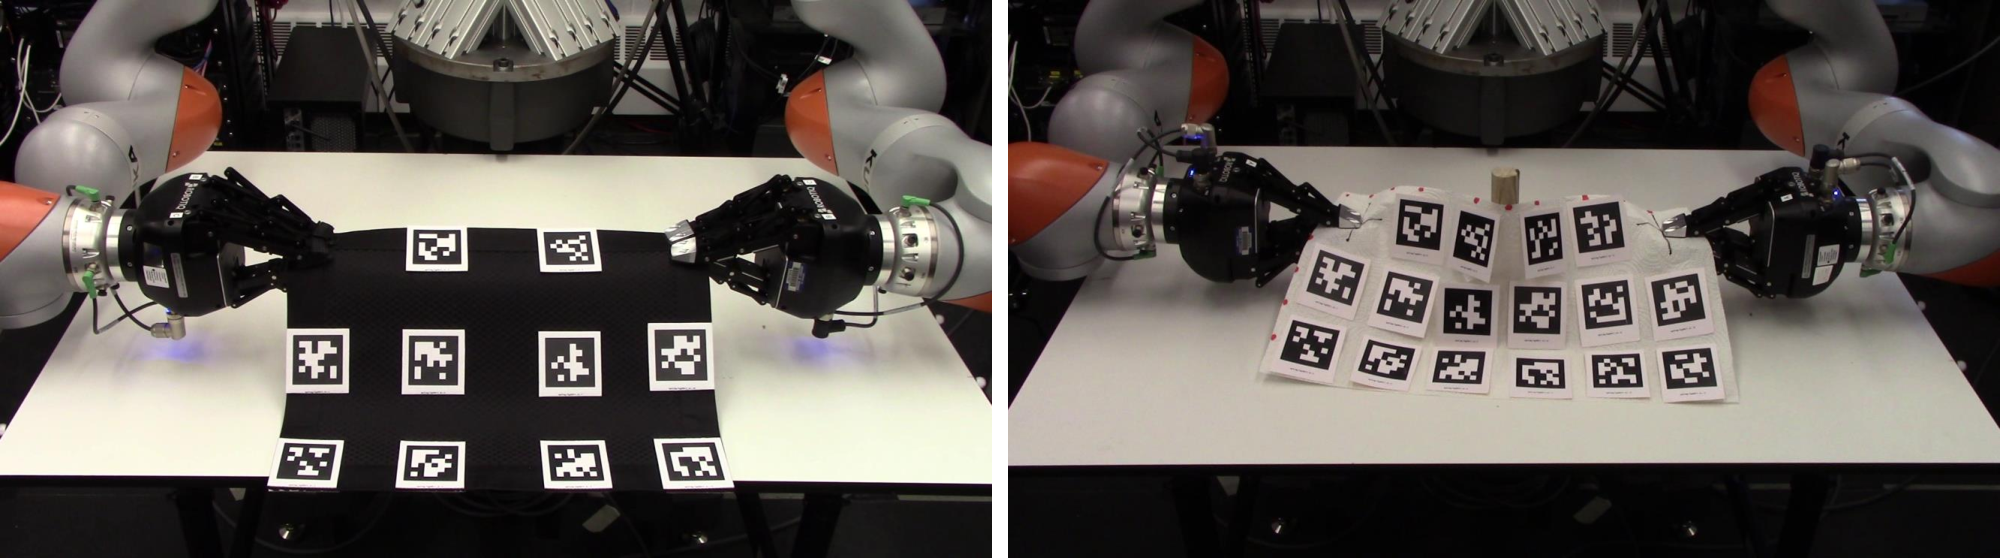
\includegraphics[width=.5\columnwidth,trim=0 0 6.7in 0,clip]{physical_robot_experiment_screenshots.pdf}
    \caption{Initial setup for the physical robot model accuracy experiment.}
    \label{fig:physical_experiment_screenshots}
\end{figure}

To evaluate our new model on a physical system, we set up an experiments with cloth-like objects manipulated by two 7DoF KUKA iiwa arms (Fig.~\ref{fig:physical_experiment_screenshots}). To sense the position of the cloth, we use the AprilTags~\cite{olson2011tags} and IAI Kinect2~\cite{iai_kinect2} libraries. The parameters are set as $\drkdir = 4$, $\drkdist = 10$, $\drkrot = 10$ for the new model. This test, which evaluates model accuracy, uses a motion profile similar to the simulation accuracy tests (Fig.~\ref{fig:cloth_model_accuracies_live}). Similar to the simulation results, the new model improves performance when dragging the cloth (first and last sections of Fig.~\ref{fig:cloth_model_accuracies_live}), and is comparable during rotational motion and when the cloth is resting on edge perpendicular to the table (see video).


\begin{figure}[ht]
    \centering
    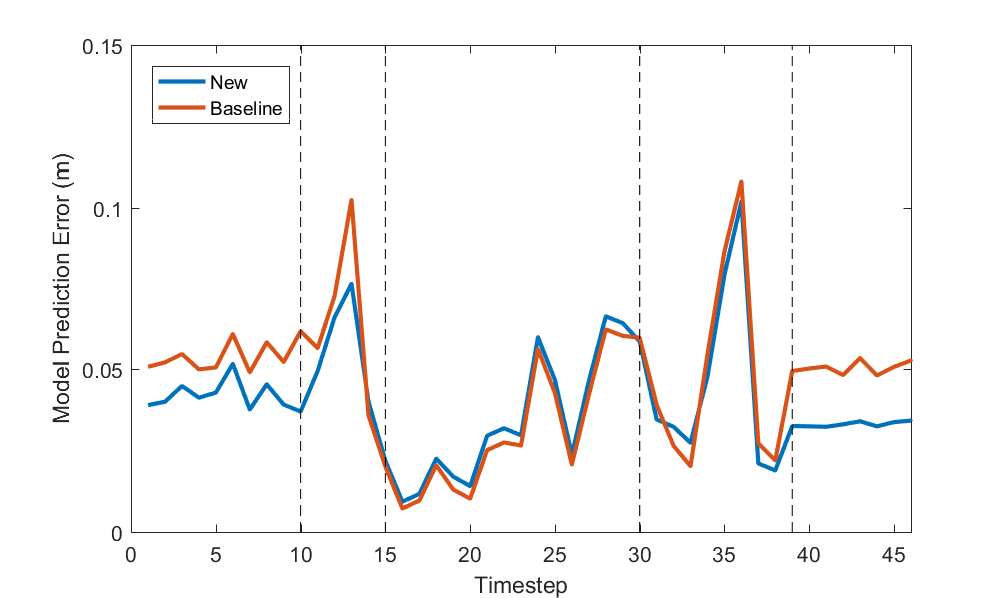
\includegraphics[width=\columnwidth]{cloth_model_accuracies_live.png}
    \caption{RMS model prediction error. The grippers pull the cloth toward the robot for the first 10 timesteps, upward for 5 timesteps, rotate for 15 timesteps, diagonally down and away for 9 timesteps, then directly away from the robot.}
    \label{fig:cloth_model_accuracies_live}
\end{figure}

\subsection{Computation Time}

\begin{table}[ht]
%\renewcommand{\arraystretch}{1.2}
\centering
\resizebox{\linewidth}{!}{
\begin{tabular}{|c|c|c|c|c|}
\hline
            & rope-wrapping & rope-matching & cloth-passing & cloth-wrapping \\
            & -cylinder     & -zig-path     & single-pole   & -two-cylinders \\
\hline
BT    & 0.686   & 0.571   & 19.29   & 3.680   \\
\hline
NM   & 0.029   & 0.014   & 1.172   & 0.339   \\
\hline
\hline
\# evals &  50.72 & 143.5 & 83.81 & 63.32\\
\hline
\end{tabular}
}
\caption{Top two rows: Mean computation time (ms) per model prediction for a given gripper motion. BT: Bullet simulator; NM: new model. Bottom row: Mean number of times the model was evaluated when executing the controller in Sec.~\ref{sec:stretching_constraint_controller}.}
\label{tbl:simulation_time_report}
\end{table}

\todo{Use consistent table format throughout}

\todo{Clean up this wording and cross referencing, probably by using a single complied results section.}
To verify the practicality of our method, we gathered data comparing its computation time to the benchmark's and to using the Bullet simulator for a variety of tasks (see Sec.~\ref{sec:stretching_constraint_controller_results}). Table~\ref{tbl:simulation_time_report} shows a comparison between the average time needed to evaluate the new model and the time needed to simulate a gripper motion with the Bullet simulator; Table~\ref{tbl:controller_time_report} shows a comparison between the combination of this model and the controller in Sec.~\ref{sec:stretching_constraint_controller}. Note that the amount of time required for the simulator to converge to a stable estimate depends on many conditions, including what object is being simulated. Through experimentation we determined that 4 simulation steps were adequate for rope and 10 for cloth. Comparing the time needed to do this simulation to the time needed to evaluate our model, we see that the new model is indeed faster by at least an order of magnitude, in some cases by two orders of magnitude, confirming that, despite being slower than the benchmark, our method still outperforms the simulator in terms of computation time.



